\documentclass[a4paper]{article}

\usepackage[english]{babel}
\usepackage[utf8x]{inputenc}
\usepackage{amsmath}
\usepackage{graphicx}
\usepackage{float}
\usepackage[colorinlistoftodos]{todonotes}
\usepackage{subfig}

\title{Assignment 2 - Intelligent Multimedia Systems}
\author{R\'emi de Zoeten (6306894) and Anouk Visser (6277209)}

\begin{document}
\maketitle


\section{Introduction}
Our assignment was to use Gaussian image filters and Gaussian derivatives to manipulate images. This can be used to find edges in images and an orientation of those edges. 

\section{Results}
\subsection{Gaussian Convolutions}
We implemented the function \emph{gaussian} that produces a 1D vector that can be used to convolve an image. When called, \emph{gaussian(1)} will produce the following vector:

$$ [ 0.0044, 0.0540, 0.2420, 0.3991, 0.2420, 0.0540, 0.0044 ] $$

When plotting the resulting vector using MATLAB's \emph{plot} it is clear that the function indeed produces a Gaussian. The plots can be seen in figure \ref{gauss}.

\begin{figure}[H]
  \centering
  \subfloat[]{
    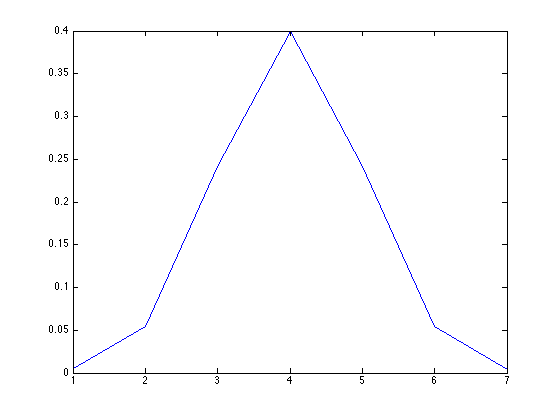
\includegraphics[width=0.5 \textwidth]{gaussSigma1.png}
    \label{sigma1}
    }
      \subfloat[]{
    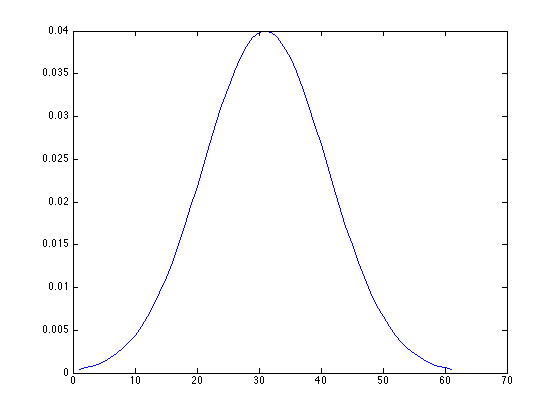
\includegraphics[width=0.5 \textwidth]{gaussSigma10.png}
    \label{sigma10}
    }
  \caption{\subref{sigma1} shows the plot of the result of \emph{gaussian(1)}. \subref{sigma10} shows the result of the same function with $\sigma = 10$. }
  \label{gauss}
\end{figure}

\noindent
Using the function \emph{gaussian} we can apply a Gaussian filter in both the $x$ and $y$ direction to an image. In figure \ref{fig:blurredZebra} we can see the results for two different combinations of sigma.
\begin{figure}[H]
  \centering
    \subfloat[]{
    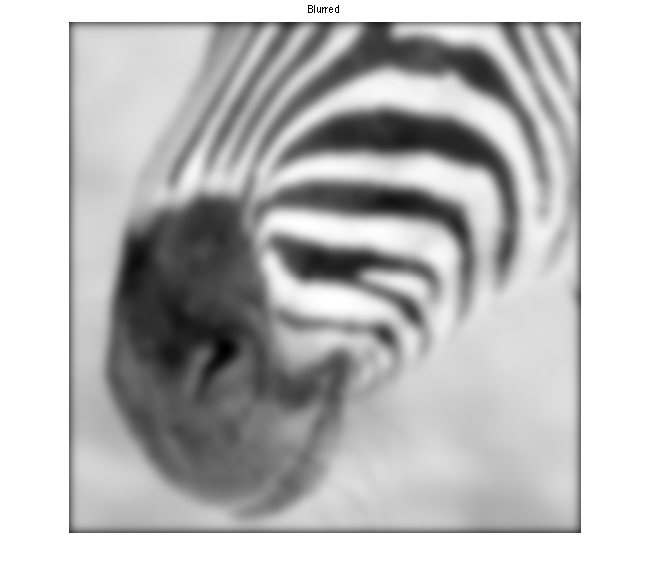
\includegraphics[width=0.50 \textwidth]{gaussianConv5.png}
    \label{blur5}
   }
  \subfloat[]{
    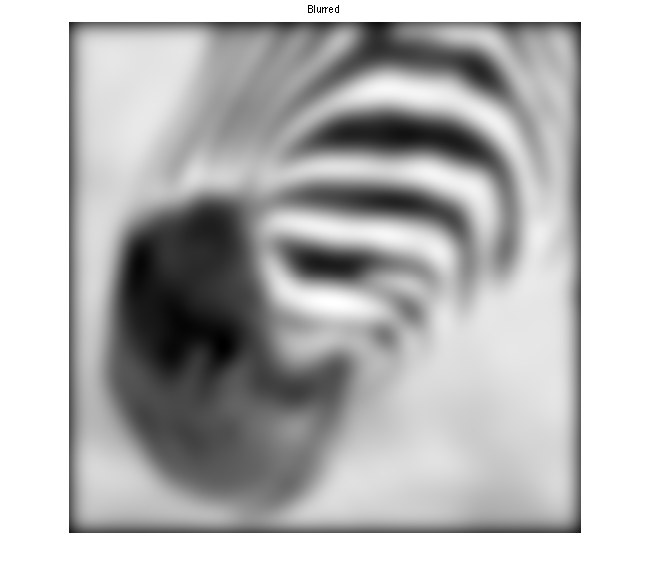
\includegraphics[width=0.50 \textwidth]{gaussianConv.png}
    \label{blur10}
   }
  \caption{Results of convolving an image along the x-axis and the y-axis separately with a 1D Gaussian as produced by \emph{gaussian}. \subref{blur5} shows the result obtained by using a 1D Gaussian with $\sigma = 5$ in both directions. \subref{blur10} shows the result obtained by using a 1D Gaussian with $\sigma = 10$ in both directions. }
  %seperability
  \label{fig:blurredZebra}
\end{figure}

When using MATLAB's built-in functions to perform a Gaussian convolution with $\sigma = 10$ (MATLAB convolve the image with a 2D Gaussian filter), then the results are not numerically identical. However, the difference is not visible and the sum of the differences per pixel is 1.7433e-10 and the average difference per pixel is 6.6503e-16.\\

\subsection{Gradient Magnitude and Orientation}

We implemented the function \emph{gaussianDer} that produces a 1D vector that can be used to convolve an image. When plotting the resulting vector using MATLAB's \emph{plot} we see the shape of the expected Gaussian derivative. The plots can be seen in figure \ref{gaussDer}.

\begin{figure}[H]
  \centering
  \subfloat[]{
    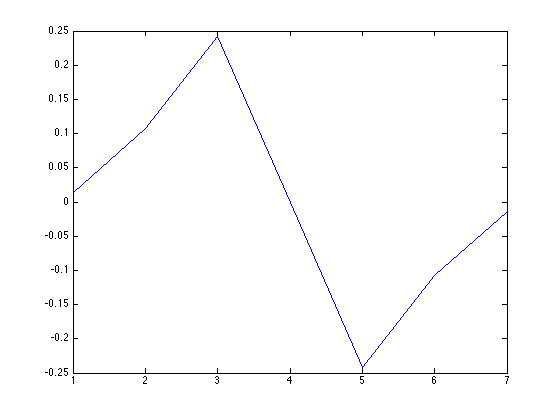
\includegraphics[width=0.5 \textwidth]{gaussDer1.png}
    \label{sigma1}
    }
      \subfloat[]{
    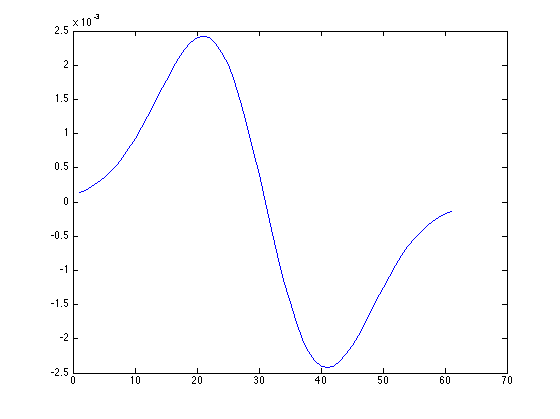
\includegraphics[width=0.5 \textwidth]{gaussDer10.png}
    \label{sigma10}
    }
  \caption{\subref{sigma1} shows the plot of the result of \emph{gaussianDer} with $\sigma = 1$. \subref{sigma10} shows the result of the same function with $\sigma = 10$. }
  \label{gaussDer}
\end{figure}

Using the derivative of the Gaussian we can determine the the magnitude and orientation of the gradient for each pixel of an input image. Figure \ref{magOr} shows the results for three different values of sigma. 

\begin{figure}[H]
  \centering
  \subfloat[]{
    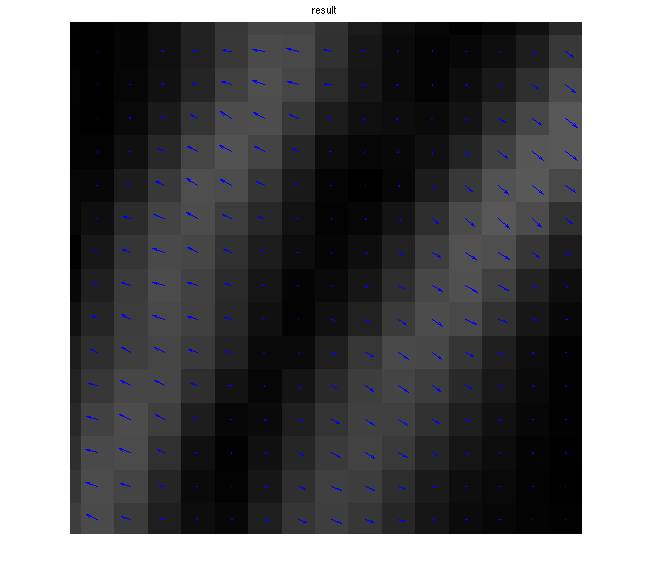
\includegraphics[width=0.35 \textwidth]{zoom1.png}
   }
   \subfloat[]{
    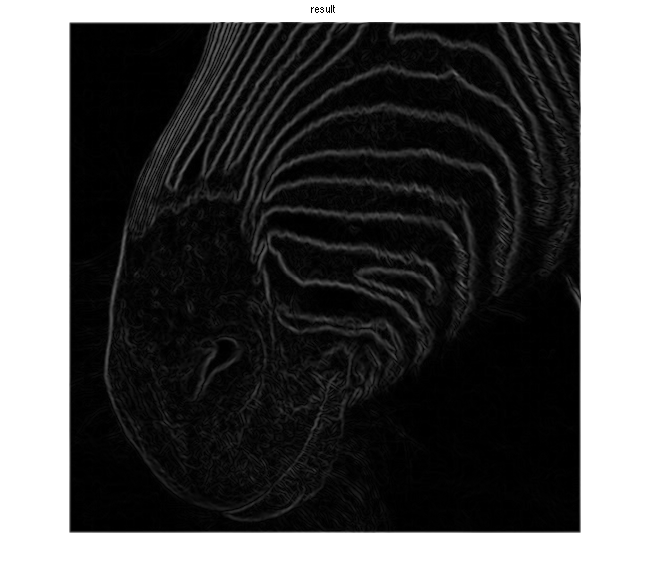
\includegraphics[width=0.35 \textwidth]{mag1.png}
   }
      \subfloat[]{
    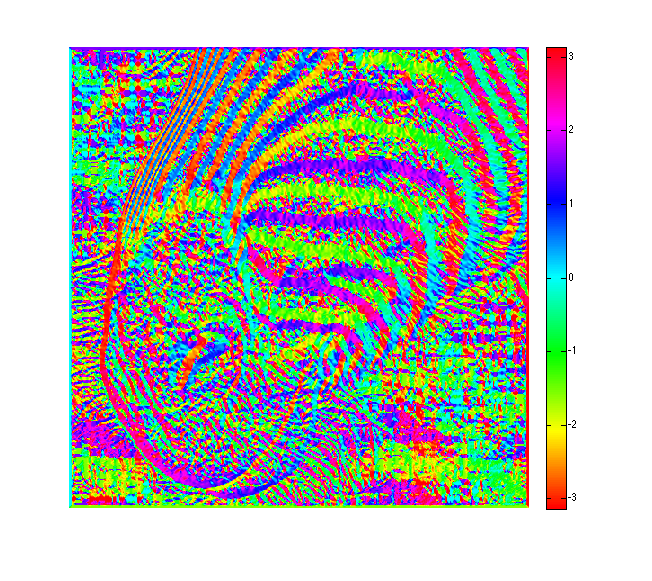
\includegraphics[width=0.35 \textwidth]{or1.png}
   }\\
     \subfloat[]{
    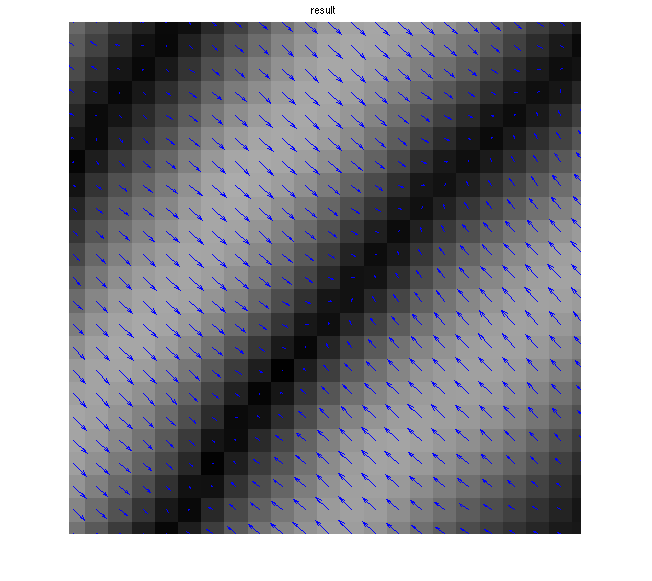
\includegraphics[width=0.35 \textwidth]{zoom5.png}
   }
   \subfloat[]{
    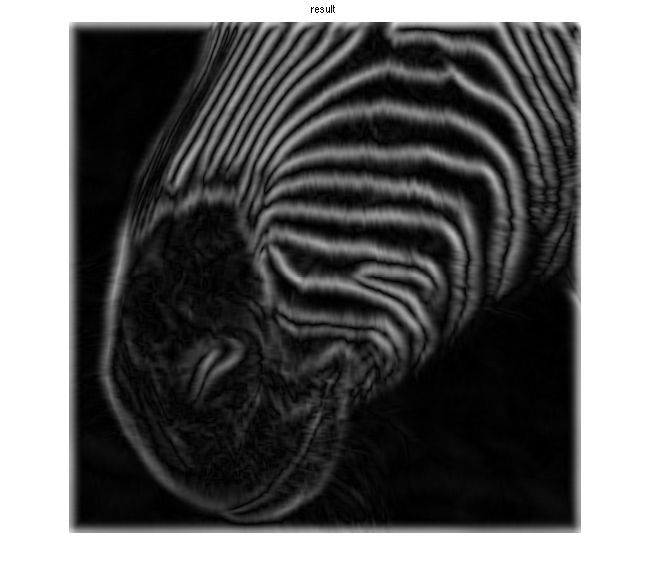
\includegraphics[width=0.35 \textwidth]{mag5.png}
   }
      \subfloat[]{
    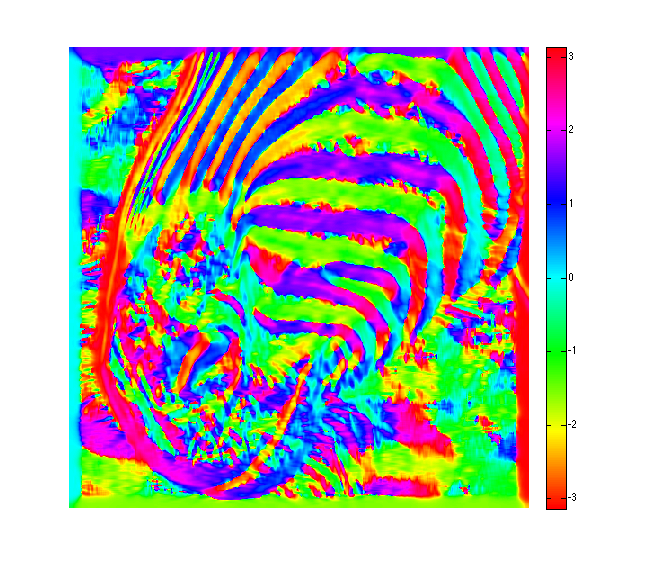
\includegraphics[width=0.35 \textwidth]{or5.png}
   }\\
     \subfloat[]{
    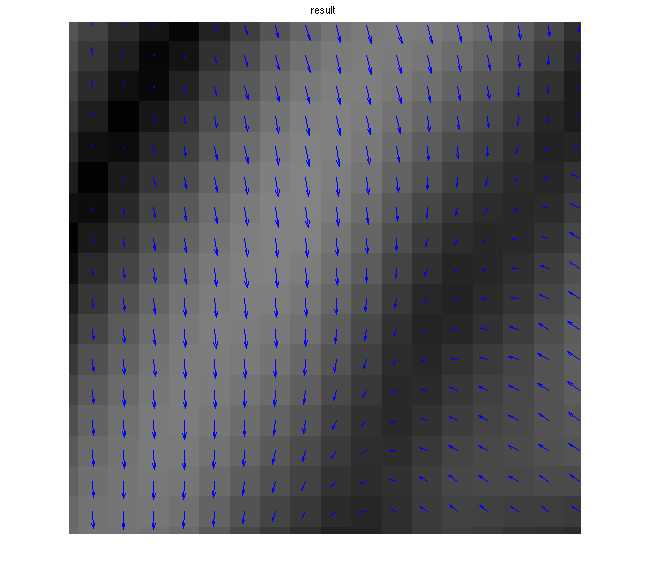
\includegraphics[width=0.35 \textwidth]{zoom10.png}
   }
   \subfloat[]{
    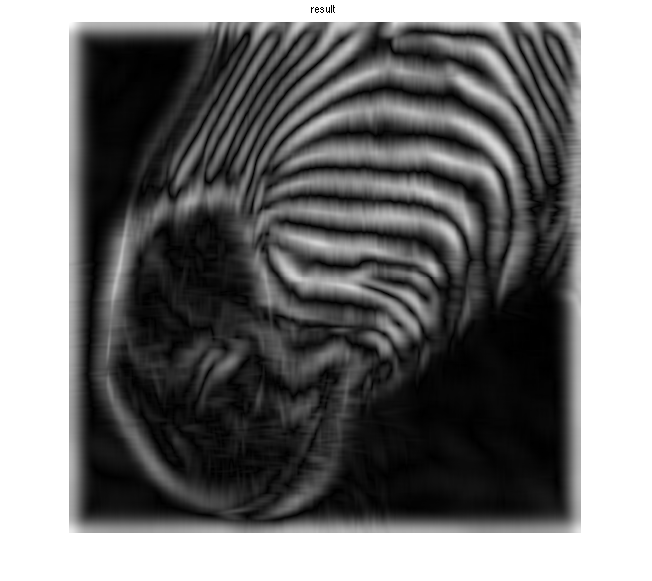
\includegraphics[width=0.35 \textwidth]{mag10.png}
   }
      \subfloat[]{
    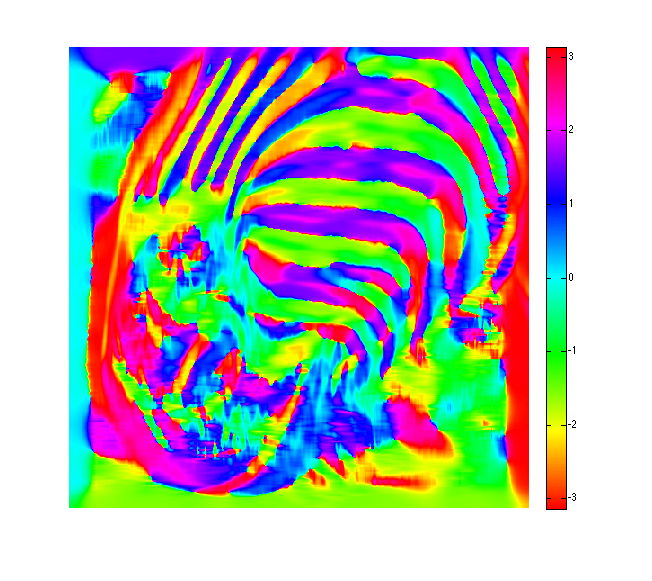
\includegraphics[width=0.35 \textwidth]{or10.png}
   }
  \caption{The images were sampled using the following sigma values: a-c: $\sigma  = 1$, d - f: $\sigma = 5$, g-i: $\sigma=10$. The magnitude images become more clear or white as the sigma increases. The colored orientation images become more regular as the sigma increases, because small local variances even out when a larger sigma is used.}
     \label{magOr}
\end{figure}

\noindent
We have applied a binary filter to the magnitude images for the sigma's $\{1,5,10\}$ and threshold values $\{0.025, 0.02, 0.013\}$. The results of this can be viewed in figure \ref{fig:mag9}.

\begin{figure}[H]
  \centering
    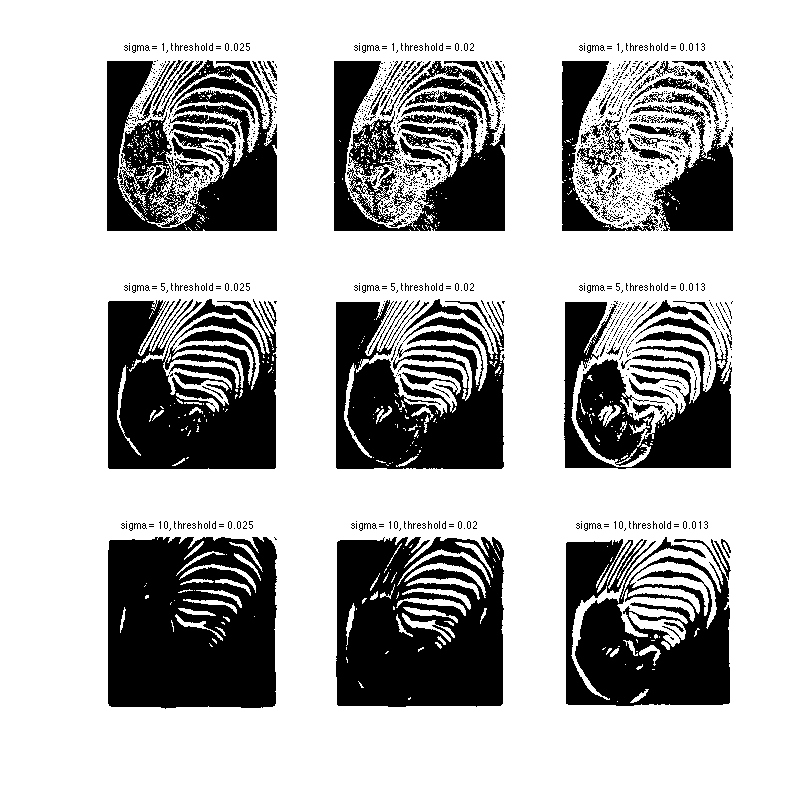
\includegraphics[width=1 \textwidth]{mag9.png}
  \caption{Binariry magnitude images. Choosing an appropriate threshold value is dependent on the sigma that is used. A larger sigma requires a lower threshold.}
  \label{fig:mag9}
\end{figure}


\subsection{Second Order Gaussian Derivative}
We implementend the function \emph{gaussianDer(G,sigma)} and used it along with \emph{gaussian(sigma)} to implement the function \emph{ImageDerivatives(img,sigma,type)}.
The following figures show images that were created using the \emph{ImageDerivatives} script and $\sigma=20$. The input image (figure \ref{fig:dot}) was a black $201 \times 201$ pixel image with the center pixel white.

\begin{figure}[H]
  \centering
    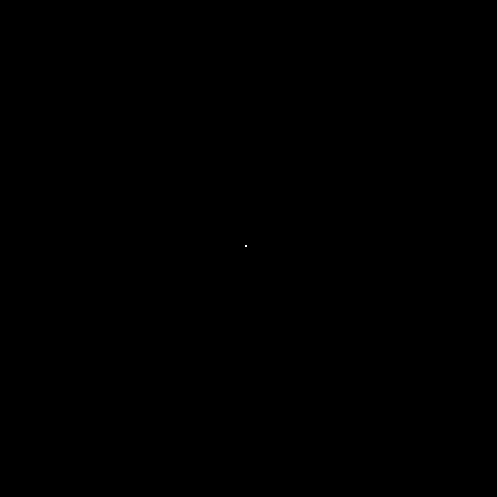
\includegraphics[width=0.45 \textwidth]{dot.png}
  \caption{Impulse image.}
  \label{fig:dot}
\end{figure}


\begin{figure}[H]
  \centering
    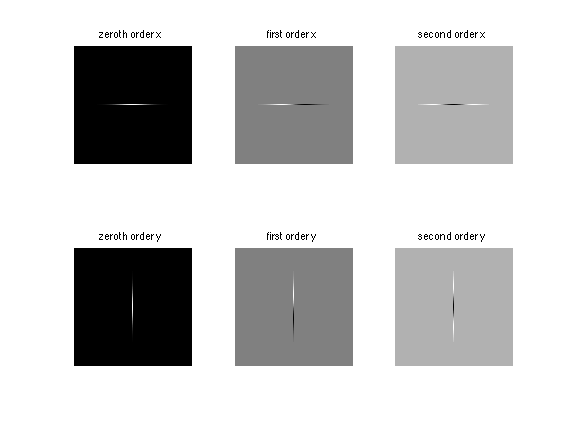
\includegraphics[width=0.95 \textwidth]{xy.png}
  \caption{Zeroth, first and second order Gaussian derivatives of the impulse image shown separately in the x and the y direction.}
  \label{fig:dot}
\end{figure}

\begin{figure}[H]
  \centering
    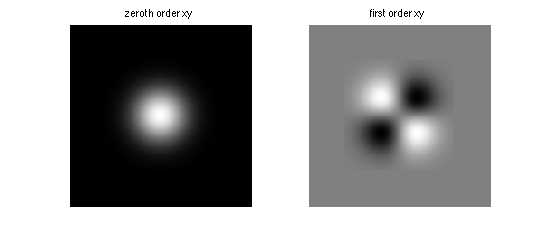
\includegraphics[width=0.95 \textwidth]{new.png}
  \caption{Zeroth and first order Gaussian derivatives of the impulse image applied in both the x and the y direction.}
  \label{fig:dot}
\end{figure}

\section{Conclusion}
In this assignment we have implemented a 1D discrete Gaussian filter and used it to convolve it with an image in the x and y direction separately, resulting in a blurred image. We have shown that using a separate kernel we obtain the same results as the built-in MATLAB functions, which use a 2D Gaussian filter. \\
Using the first order Gaussian derivative and convolving this with the image, we have created images showing the image's gradient and magnitude for each pixel. When a threshold is applied to the magnitude image, we obtain a binary image showing the edges that depend on the threshold chosen.\\\
Finally, we applied different 1D Gaussian derivative filters on an impulse image. 







\end{document}





